\documentclass[a4paper,draft]{report} % 或用 \documentclass[UTF8]{ctexrep}
\usepackage[margin=1.25in]{geometry}
\usepackage[UTF8]{ctex} % 中文支持
\usepackage{listings}
\usepackage{xcolor}
\usepackage{tabularx} % 自适应宽度表格
\usepackage{array}    % 表格格式增强
\usepackage{booktabs} % 更漂亮的横线
\usepackage{hyperref}
\usepackage{amsmath, amssymb} % 数学符号支持
\usepackage{bm} % 粗体数学符号
\usepackage{graphicx} %插入图片的宏包
\usepackage{float} %设置图片浮动位置的宏包
\usepackage{subcaption}
\usepackage{enumitem}

\hypersetup{
    colorlinks=true,
    linkcolor=black,
    filecolor=magenta,
    urlcolor=cyan
}

\newcommand{\enabstractname}{Abstract}
\newcommand{\cnabstractname}{摘要}
\newenvironment{enabstract}{%
  \par\Large
  \noindent\mbox{}\hfill{\bfseries \enabstractname}\hfill\mbox{}\par
  \vskip 2.5ex}{\par\vskip 2.5ex}
\newenvironment{cnabstract}{%
  \par\Large
  \noindent\mbox{}\hfill{\bfseries \cnabstractname}\hfill\mbox{}\par
  \vskip 2.5ex}{\par\vskip 2.5ex}

\definecolor{codegray}{gray}{0.98}
\definecolor{codepurple}{rgb}{0.58,0,0.82}
\lstdefinestyle{mystyle}{
    backgroundcolor=\color{codegray},   
    commentstyle=\color{gray},
    keywordstyle=\color{blue},
    numberstyle=\tiny\color{gray},
    stringstyle=\color{codepurple},
    basicstyle=\ttfamily\small,
    breaklines=true,                 
    captionpos=b,                    
    keepspaces=true,                 
    numbers=left,                    
    numbersep=5pt,                  
    showspaces=false,                
    showstringspaces=false,
    showtabs=false,                  
    tabsize=4
}
\lstset{style=mystyle, language=Python}

\setcounter{tocdepth}{1} 

\title{基于布朗粒子运动的微小位移测量实验设计与验证}
\author{E}
\date{\today}

\begin{document}
\maketitle

\begin{cnabstract}
\large
  
热力学基本规律在宏观体系中已得到广泛验证,但其在微观尺度下的适用性仍需深入探讨。
本研究以布朗运动为典型模型,结合高精度离轴全息技术与理论分析,从微观粒子的热运动出发,系统研究了不可逆过程中的熵产生机制。
实验通过离轴全息光路实时追踪布朗粒子的随机位移,利用干涉条纹与相位反演实现微球位置的高分辨率测定,从而精确统计其扩散行为与能量涨落特性。
基于此,我们建立了布朗运动中扩散系数与熵产生率之间的定量关系,验证了微观尺度下热力学不确定关系的普适性,揭示了非平衡态统计规律与热力学第二定律的内在一致性。
进一步通过熵产生率的时空分布分析,阐明了微观热运动的不可逆性及其与宏观热力学的关联机制。本研究不仅为离轴全息技术在微纳尺度热力学测量中的应用提供了一种思路,
还为从微观层面验证热力学基本规律提供了实验依据,对理解非平衡态统计物理与微纳系统能量耗散机制具有重要意义。
\par\textbf{关键字: } 布朗运动,熵产生率,热力学不确定关系,离轴全息
\end{cnabstract}

\newpage
\begin{enabstract}
\large
The basic laws of thermodynamics have been widely verified in the macro system, but its applicability at the micro scale still needs to be further explored.
Based on the thermal motion of microscopic particles, this experiment takes Brownian motion as a typical model, and combines experimental and theoretical analysis.
By measuring the random displacement behavior of Brownian particles, the entropy generation mechanism in irreversible process is verified.
Furthermore, we establish the thermodynamic uncertainty relationship between diffusion coefficient and entropy generation in Brownian motion.
The statistical law behind microscopic thermal motion and its consistency with the second law of thermodynamics are revealed.
This experimental study provides an effective way to verify the basic laws of thermodynamics from the microscopic scale.
It is of great significance to understand the thermodynamic behavior of micro-system in non-equilibrium state.
\par\textbf{Keywords:} Brownian motion, entropy production rate, thermodynamic uncertainty relation, off-axis holography
\end{enabstract}

\tableofcontents

\chapter{题意解析}
\section{题目}
这里是section部分
\subsection{目的}
这里是subsection部分

\chapter{实验原理}
\section{有效动能温度公式推导}

考虑被光阱束缚的布朗粒子运动,在自由粒子近似下忽略势能项,其朗之万方程为:
\begin{equation}
m \frac{dv}{dt} = -\gamma v + \xi(t) + \zeta(t),
\end{equation}
其中:
\begin{itemize}
    \item $v = \dot{x}$ 为粒子速度;
    \item $\xi(t)$ 为热噪声,对应环境温度 $T_w$;
    \item $\zeta(t)$ 为外部随机力,振幅为 $\sigma$。
\end{itemize}

噪声的统计特性如下:
\begin{align}
\langle \xi(t) \xi(t') \rangle &= 2\gamma k T_w \,\delta(t - t'), \\
\langle \zeta(t) \zeta(t') \rangle &= \sigma^2 \,\delta(t - t'), \\
\langle \xi(t) \zeta(t') \rangle &= 0.
\end{align}

定义总噪声 $\eta(t) = \xi(t) + \zeta(t)$,其自相关函数为:
\begin{equation}
\langle \eta(t) \eta(t') \rangle = \big( 2\gamma k T_w + \sigma^2 \big) \delta(t - t').
\end{equation}

朗之万方程的稳态解为:
\begin{equation}
v(t) = \frac{1}{m} \int_{-\infty}^{t} e^{-\frac{\gamma}{m}(t-\tau)} \eta(\tau) \, d\tau.
\end{equation}

计算速度方差:
\begin{align}
\langle v^2(t) \rangle &= \frac{1}{m^2} \int_{-\infty}^{t} \!\! \int_{-\infty}^{t} 
e^{-\frac{\gamma}{m}(t-\tau)} e^{-\frac{\gamma}{m}(t-\tau')} 
\langle \eta(\tau) \eta(\tau') \rangle \, d\tau \, d\tau' \notag \\
&= \frac{2\gamma k T_w + \sigma^2}{m^2} \int_{-\infty}^{t} e^{-\frac{2\gamma}{m}(t-\tau)} \, d\tau \notag \\
&= \frac{2\gamma k T_w + \sigma^2}{2\gamma m}.
\end{align}

根据能量均分定理:
\begin{equation}
\frac{1}{2} m \langle v^2 \rangle = \frac{1}{2} k T_{\text{kin}},
\end{equation}
代入上式可得:
\begin{equation}
T_{\text{kin}} = T_w + \frac{\sigma^2}{2k\gamma}.
\end{equation}

因此,外部随机力会等效提高布朗粒子的有效动能温度,其增加量与噪声强度平方成正比,与阻尼系数成反比。

\section{噪声强度与扩散系数的修正关系}

\subsection{噪声强度的定义}
从朗之万方程的过阻尼形式出发:
\begin{equation}
\gamma \dot{x} = f(x,t) + \eta(t),
\end{equation}
其中 $\gamma$ 为摩擦系数,$\eta(t)$ 为零均值随机噪声,其完整统计特性为:
\begin{equation}
\langle \eta(t)\eta(t') \rangle = \big( 2\gamma k_B T_w + \sigma^2 \big) \, \delta(t-t'),
\end{equation}
其中第一项为热噪声,第二项为外加电场噪声。

\subsection{扩散系数的推导}
根据随机微分方程理论:
\begin{equation}
D = \frac{2\gamma k_B T_w + \sigma^2}{2\gamma^2}.
\end{equation}
将第一项识别为 Einstein 关系:
\begin{equation}
D = \frac{k_B T_w}{\gamma} + \frac{\sigma^2}{2\gamma^2}.
\end{equation}

\subsection{引入迁移率}
定义 $\mu \equiv 1/\gamma$,可得:
\begin{equation}
D = \mu k_B T_w + \frac{\sigma^2 \mu^2}{2}.
\end{equation}

\subsection{量纲验证}
\begin{itemize}
    \item $\gamma$: [N$\cdot$s/m](摩擦系数)
    \item $\sigma^2$: [N$^{2}\cdot$s](噪声强度)
    \item $k_B T_w$: [N$\cdot$m](热能)
\end{itemize}
检验非热噪声项的量纲:
\begin{equation}
\frac{\sigma^2}{2\gamma^2} \ \rightarrow\  \frac{\mathrm{[N^2 \cdot s]}}{\mathrm{[N^2 \cdot s^2 / m^2]}} = \mathrm{[m^2/s]},
\end{equation}
与扩散系数的量纲一致。

\subsection{熵产生率公式修正}
概率流保持原定义:
\begin{equation}
J(x,t) = \mu f(x,t)p(x,t) - D \, \partial_x p(x,t),
\end{equation}
其中 $D$ 包含了非线性项 $\sigma^2 \mu^2 / 2$。熵产生率为:
\begin{equation}
\dot{\Sigma} = \frac{1}{D} \left\langle \left( \frac{J}{p} \right)^2 \right\rangle
\geq \frac{\langle \dot{x} \rangle^2}{D}.
\end{equation}

\section{同轴全息的原理与重建}
同轴全息(In-line Holography)是最早由Gabor提出的全息记录方式,其特点是物光与参考光共轴传播,
通过干涉产生的全息图直接记录在探测平面上。该方法无需复杂的光路调整,但重建时需解决共轭像与原始像重叠的问题。
\subsection{原理}
设物光复振幅为 $O(x,y)$,同轴参考光为平面波,其复振幅可表示为
\begin{equation}
R(x,y) = A_r e^{i\phi},
\end{equation}
其中 $A_r$ 为恒定振幅,$\phi$ 为初始相位。干涉强度分布为
\begin{equation}
I(x,y) = |O(x,y) + R(x,y)|^2 = |O(x,y)|^2 + |A_r|^2 + 2A_r \text{Re}\{O(x,y)e^{-i\phi}\},
\end{equation}
其中第三项包含物光的振幅与相位信息。由于参考光与物光同轴,所有频谱成分在频域中重叠于零频附近。

\subsection{重建}
同轴全息重建需通过相位恢复算法或多次曝光法分离重叠像。典型数值重建步骤如下:
\begin{enumerate}
    \item 对全息图 $I(x,y)$ 进行二维傅里叶变换:
    \begin{equation}
    \mathcal{F}\{I(x,y)\} = \mathcal{F}\{|O|^2 + |A_r|^2\} + \mathcal{F}\{O R^*\} + \mathcal{F}\{O^* R\},
    \end{equation}
    
    \item 利用迭代相位恢复算法(如Gerchberg-Saxton算法)从重叠频谱中提取物光场 $O(x,y)$,或通过多幅不同相移的全息图分离各成分:
    \begin{equation}
    O(x,y) = \frac{1}{4A_r}\sum_{k=1}^4 I_k(x,y) e^{-i\phi_k},
    \end{equation}
    其中 $\phi_k$ 为第$k$次曝光引入的已知相移。
    
    \item 对提取的复振幅 $O(x,y)$ 进行菲涅尔衍射积分,实现物平面在任意距离 $z$ 的重构:
    \begin{equation}
    U(x,y;z) = \mathcal{F}^{-1} \left\{ \mathcal{F}[O(x,y)] \cdot e^{i 2\pi z \sqrt{\frac{1}{\lambda^2} - f_x^2 - f_y^2}} \right\}.
    \end{equation}
\end{enumerate}

同轴全息系统结构简单、光路稳定,适用于粒子场测量与微小物体成像,但需通过相位调制或算法处理解决像重叠问题。


\section{离轴全息的原理与重建}
离轴全息(Off-axis Holography)是一种通过在记录过程中引入参考光与物光的倾斜干涉来实现像分离的数字全息方法。
其核心思想是在探测面上形成包含物光波前信息的干涉条纹,并通过空间频域滤波提取所需的复振幅信息,
从而实现三维波场的数值重建。
\subsection{原理}
设物光复振幅为 $O(x,y)$,参考光复振幅为
\begin{equation}
R(x,y) = A_r e^{i 2\pi (f_x x + f_y y)},
\end{equation}
其中 $A_r$ 为参考光幅值,$f_x, f_y$ 为由倾斜角决定的空间频率分量。干涉强度分布可表示为
\begin{equation}
I(x,y) = |O(x,y) + R(x,y)|^2 = |O(x,y)|^2 + |A_r|^2 + O(x,y) R^*(x,y) + O^*(x,y) R(x,y),
\end{equation}
其中第三项和第四项分别为携带物光复振幅信息的正、共轭像调制项。

由于参考光与物光具有一定倾斜角,$O(x,y) R^*(x,y)$ 和 $O^*(x,y) R(x,y)$ 在频域中被移至原点两侧,不同于零频项 $|O|^2 + |A_r|^2$,从而可在频谱平面中利用带通滤波选取目标像的频谱区域,抑制共轭像与零级像的干扰。
\subsection{重建}
首先对干涉图 $I(x,y)$ 进行二维傅里叶变换:
\begin{equation}
\mathcal{F}\{I(x,y)\} = \mathcal{F}\{|O|^2 + |A_r|^2\} + \mathcal{F}\{O R^*\} + \mathcal{F}\{O^* R\},
\end{equation}
通过滤波保留所需的 $\mathcal{F}\{O R^*\}$ 项并进行逆傅里叶变换,可得到物光的复振幅分布(除去已知参考光相位):
\begin{equation}
O'(x,y) = \mathcal{F}^{-1} \left[ \mathcal{F}\{I(x,y)\} \cdot H(f_x,f_y) \right],
\end{equation}
其中 $H(f_x,f_y)$ 为空间频域带通滤波器。若需将物平面重构到某一距离 $z$,可利用菲涅尔衍射积分进行数值传播:
\begin{equation}
U(x,y;z) = \mathcal{F}^{-1} \left\{ \mathcal{F}[O'(x,y)] \cdot e^{i 2\pi z \sqrt{\frac{1}{\lambda^2} - f_x^2 - f_y^2}} \right\},
\end{equation}
其中 $\lambda$ 为波长,$f_x,f_y$ 为空间频率坐标。

该方法通过频域分离实现单次拍摄下的相位重建,具有结构简单、计算高效、适应性强等优点,广泛应用于显微成像、位相测量及动态过程监测等领域。

\chapter{理论模拟}

\chapter{装置设计}

\begin{figure}[H]
    \centering
    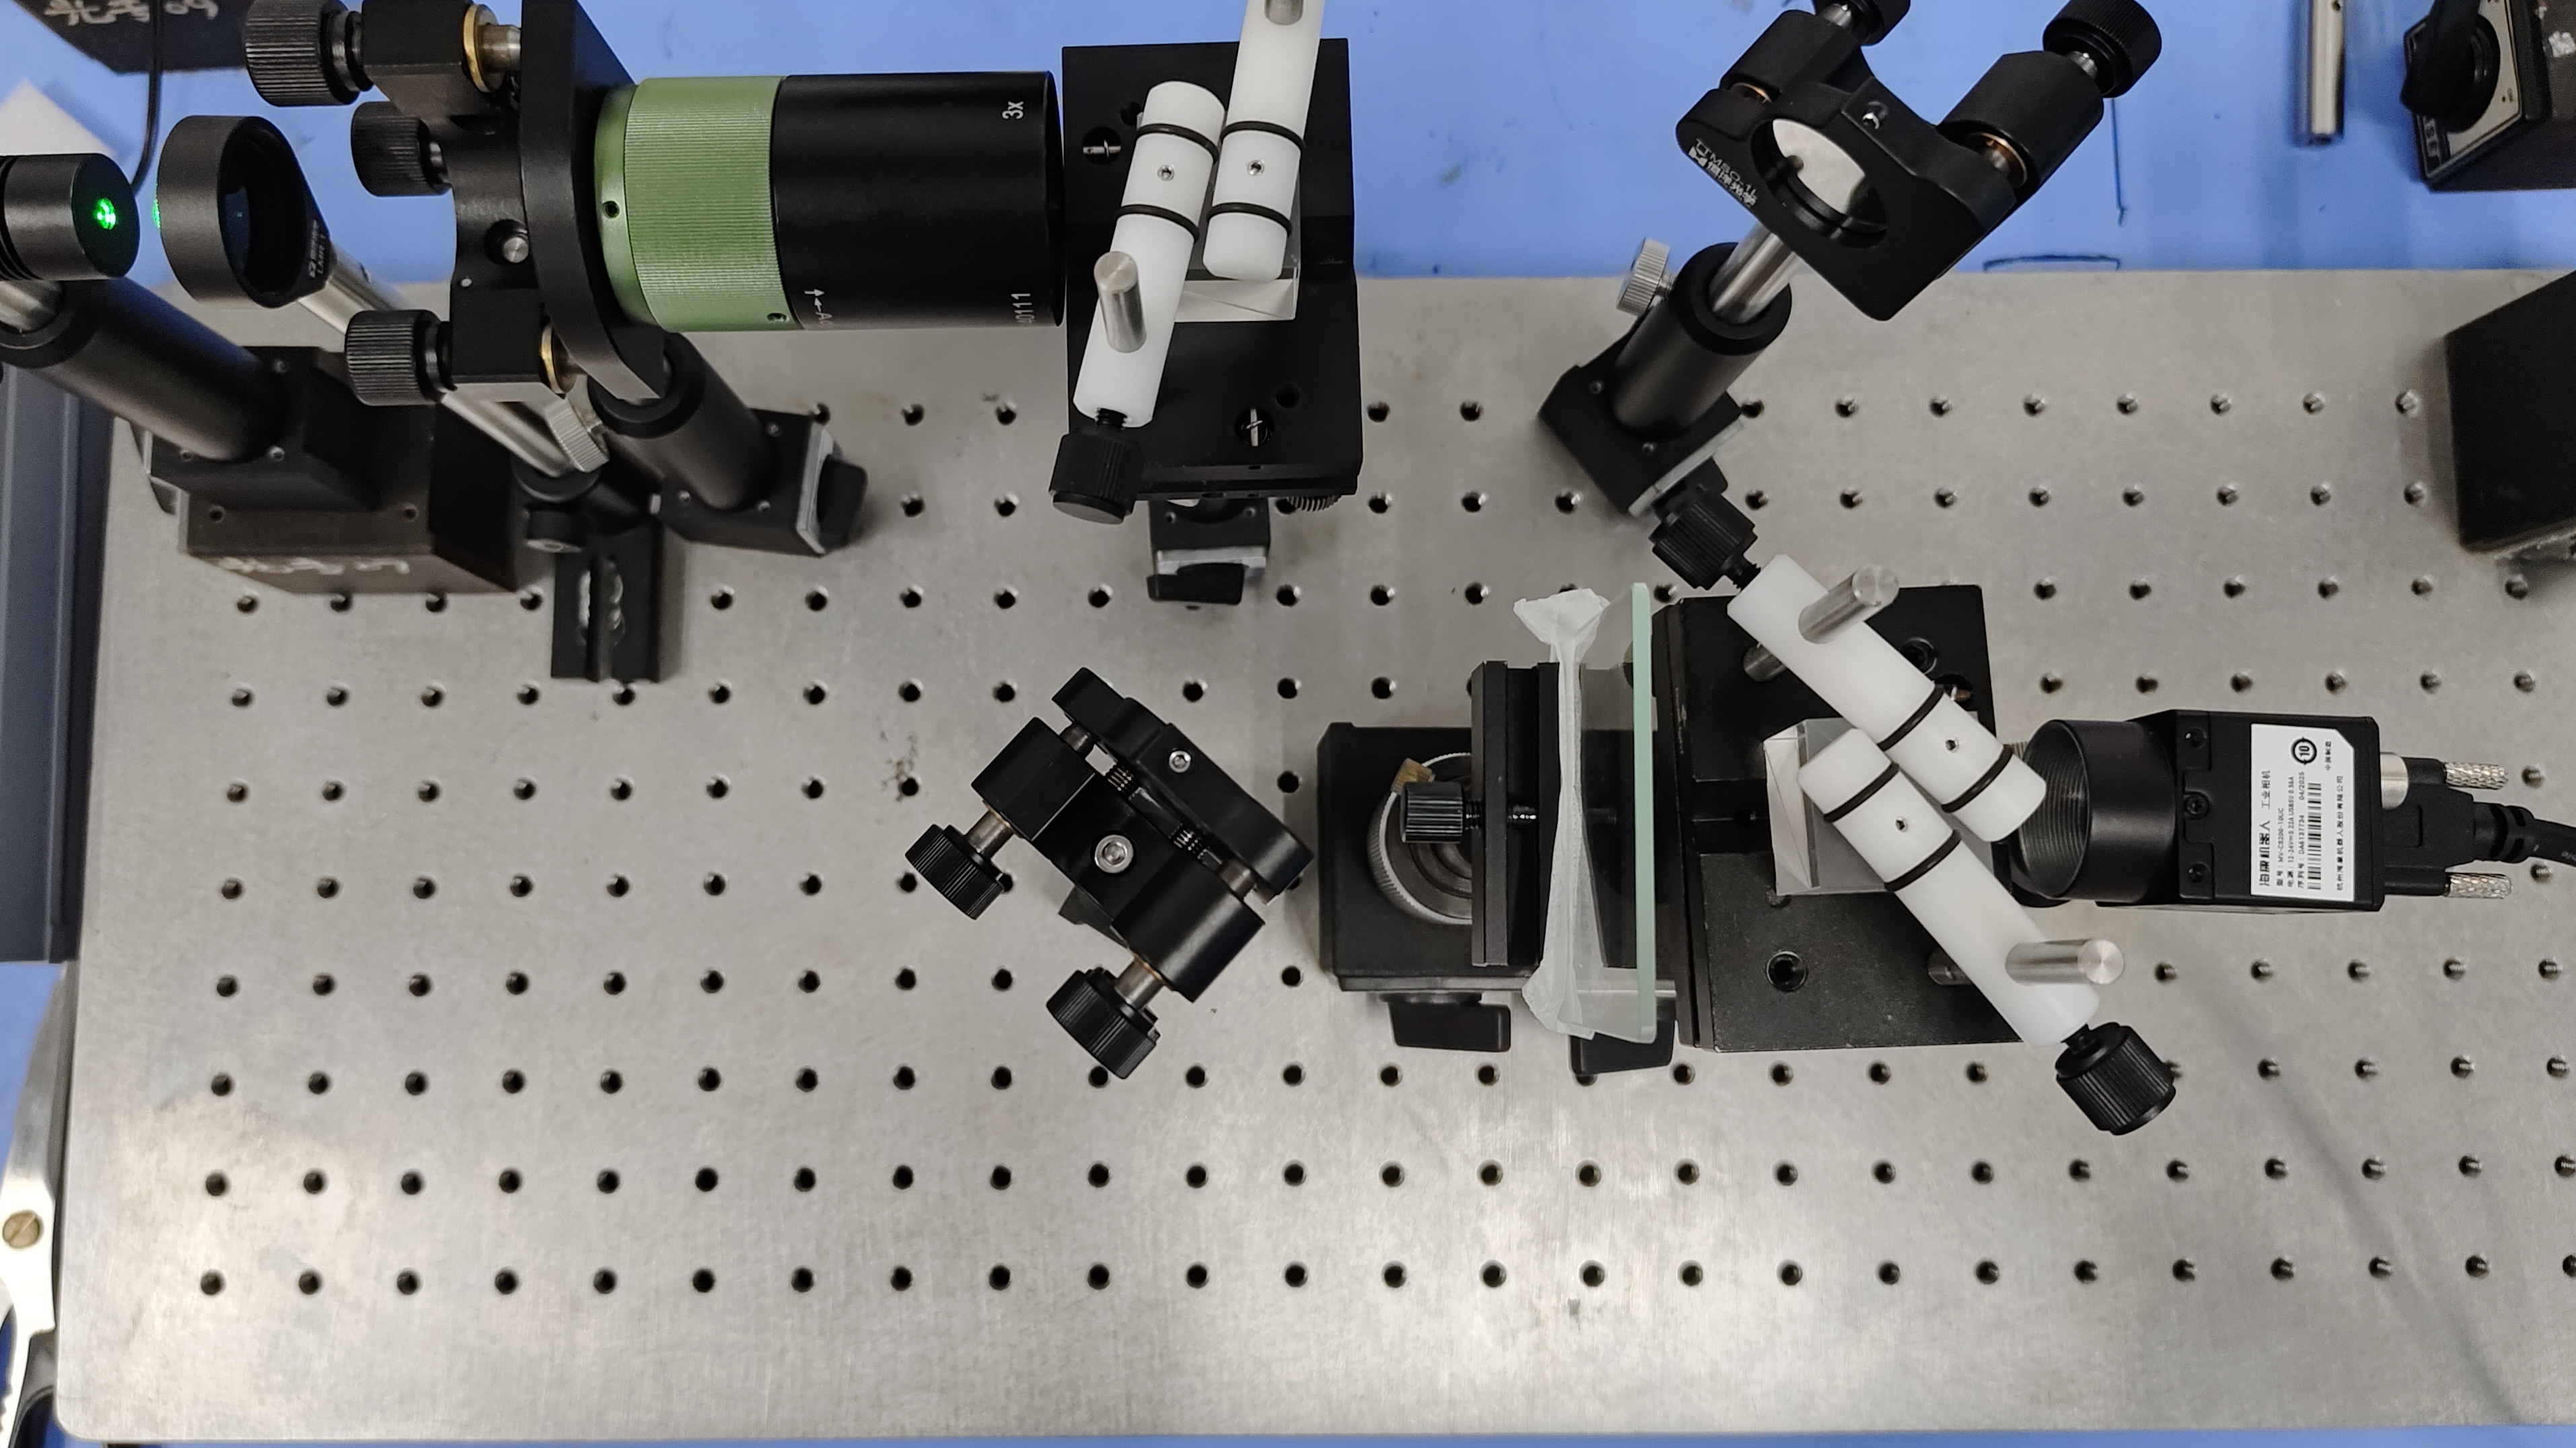
\includegraphics[width=0.9\textwidth]{expreiment}
    \caption{离轴全息实验装置示意图}
    \label{fig:experiment} % 标签名称(建议前缀 fig:)
\end{figure}

\chapter{实验内容}
\section{离轴全息确定物体位置}
\subsection{光路搭建与调试}
基于离轴全息成像原理,实验光路搭建过程如图\ref{fig:experiment}。搭建过程分为:
\textbf{光源调制}:采用波长520 nm的半导体激光器(输出功率20 mW),经扩束系统(3×扩束器)形成直径3倍扩展的平行光束。
\textbf{分光系统}:平行光束入射至第一普通分光棱镜(BS1,50:50分光比),分束为物光与参考光。物光路经反射镜M1转向后,照射分辨率板等样品,参考光路经反射镜M2反射后直接传输,两光路光程差控制在相干长度以内。最终会合在第二普通分光棱镜(BS2,50:50分光比)处,形成干涉图样。
\textbf{离轴干涉}:第二普通分光棱镜(BS2)以15°偏转角实现离轴配置,物光与参考光干涉后形成离轴全息图,由科学级CMOS相机(像素尺寸2.4 μm,5472×3648像素)记录。
通过调整CCD位置,使CCD的接收屏位于两束光的重叠处。
\subsection{拍摄全息图}
首先接通激光器电源,将CCD连接到计算机,打开相应拍摄软件。调整CCD的位置,使其处于物光和参考光完全重叠的位置。\\
然后调整CCD的曝光时间和增益,使得拍摄的全息图亮度适中,细节清晰。左右和上下移动物体(分辨率板),
使用CCD拍摄不同位置的分辨率板全息图,记录下每张全息图并保存。
\begin{figure}[H]
\centering
\begin{subfigure}{0.3\textwidth}
    \centering
    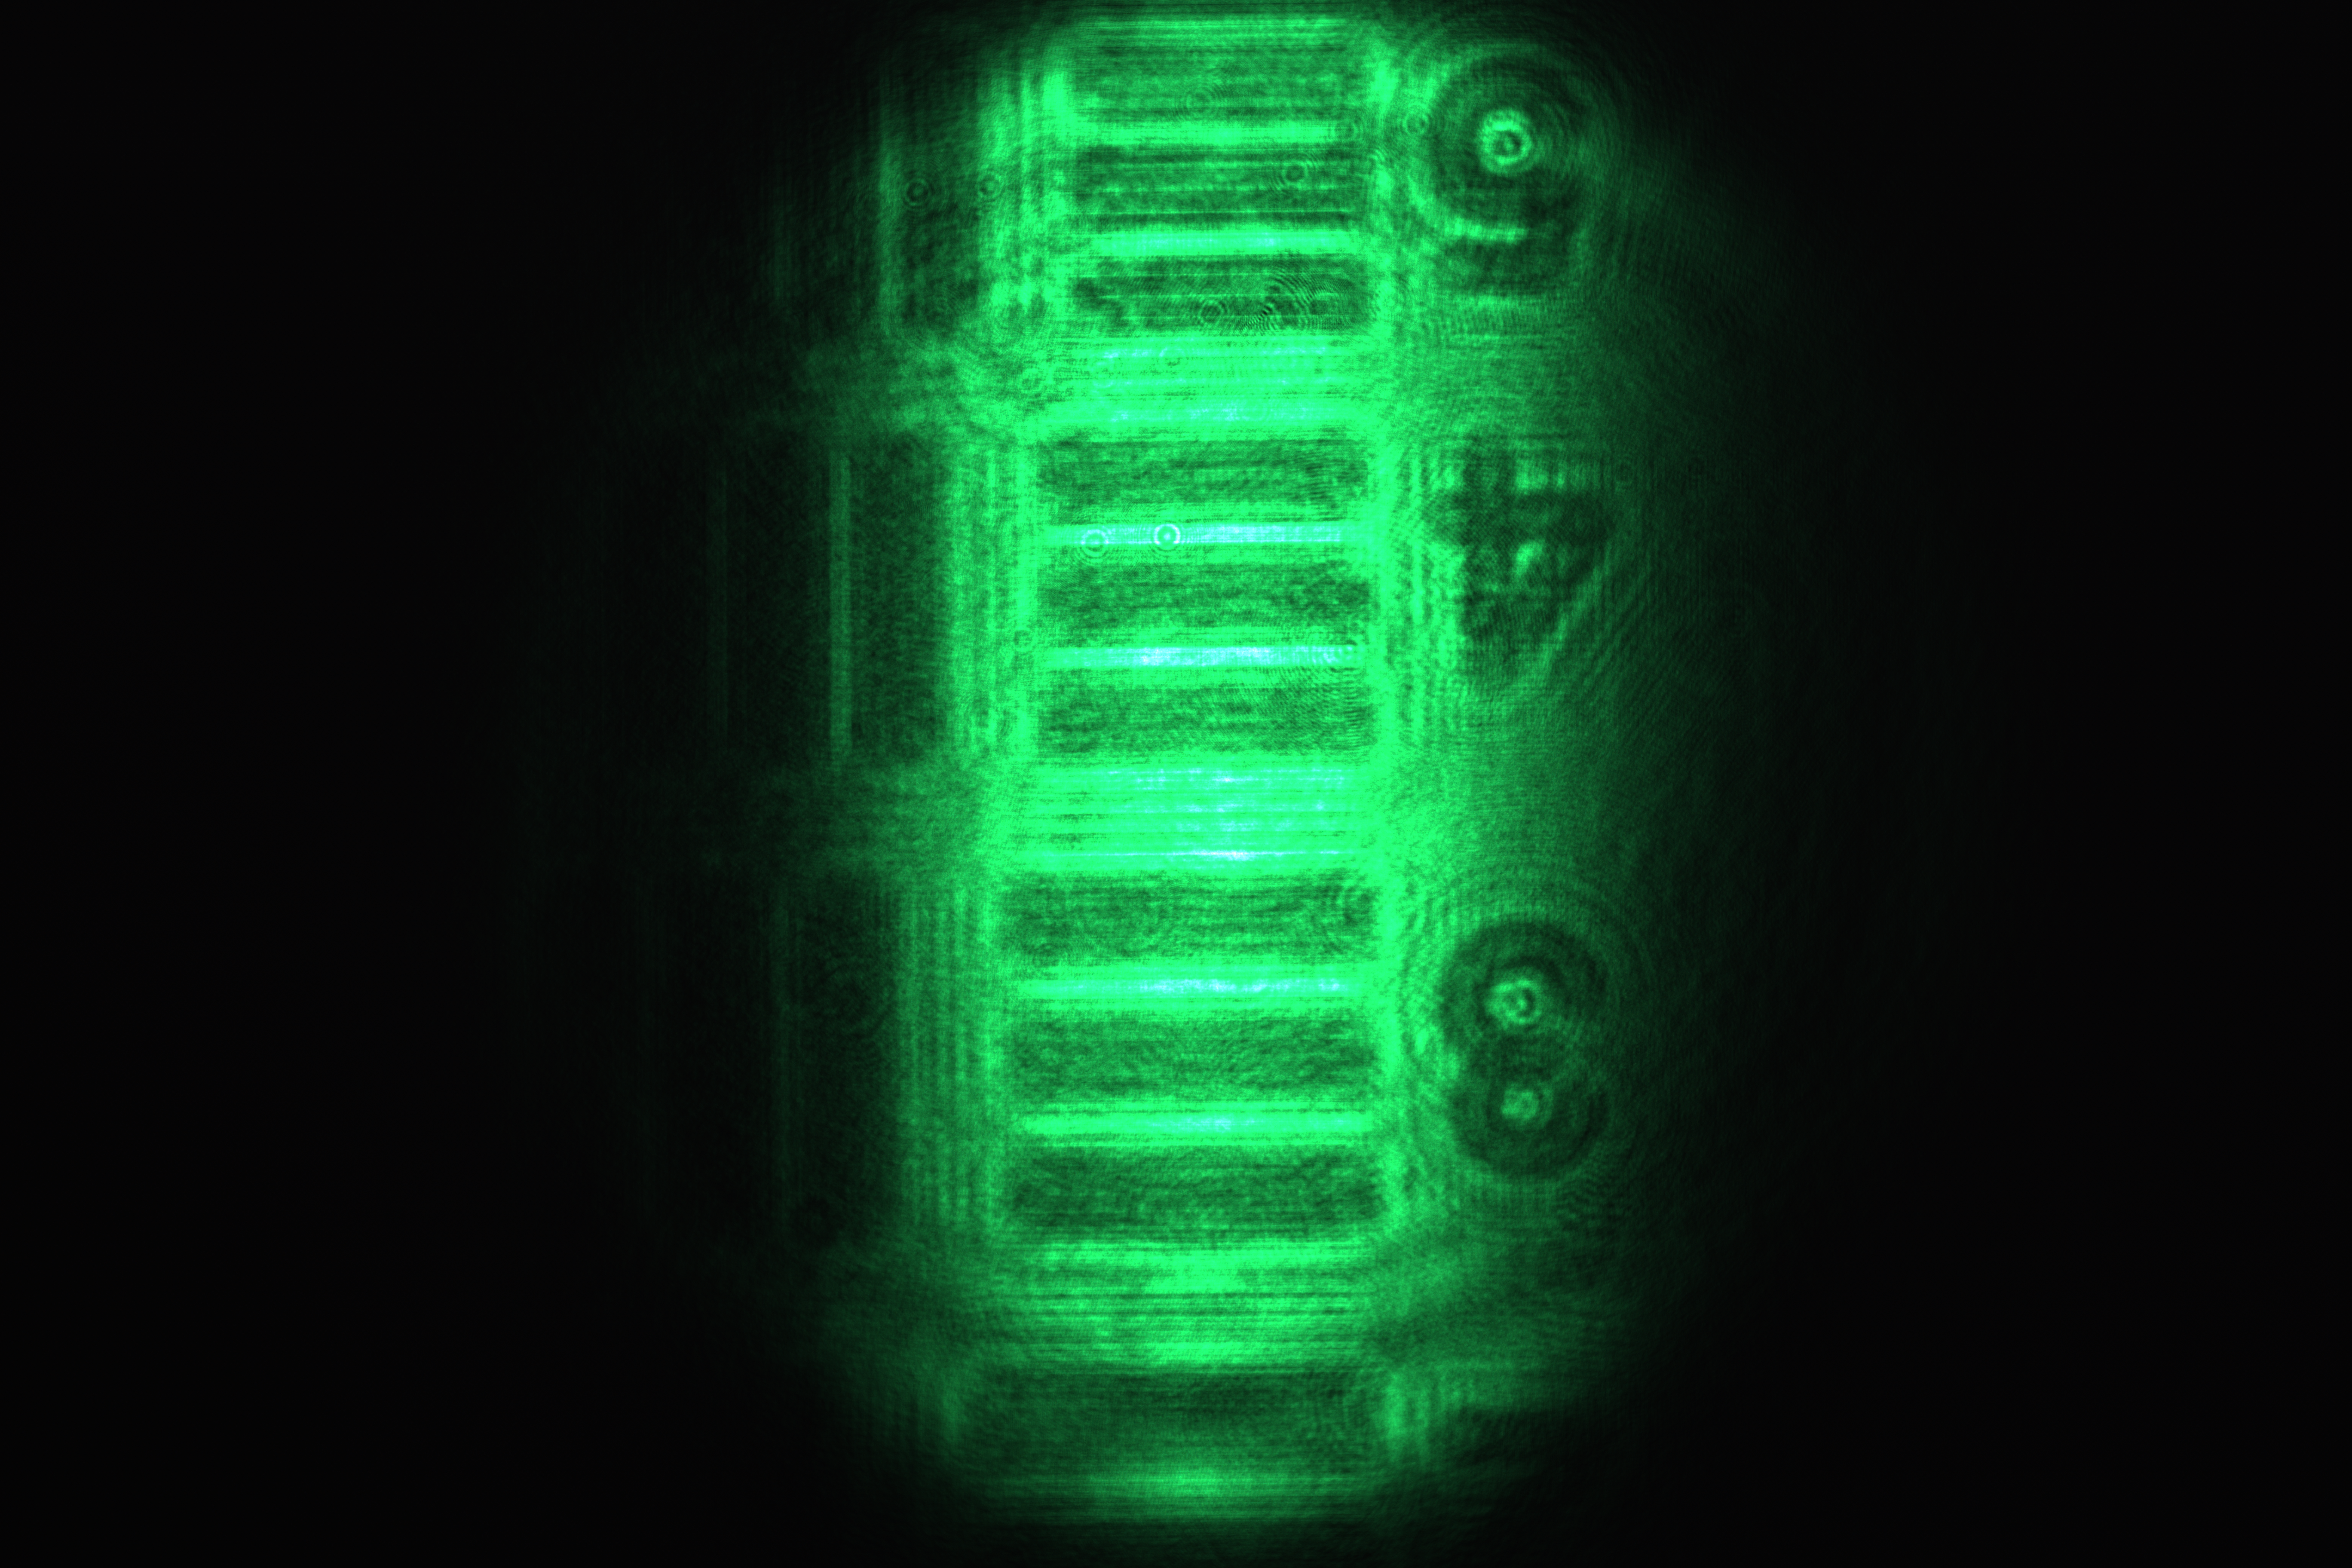
\includegraphics[width=\linewidth]{lizhou1}
    \caption{全息1}
    \label{Fig.sub.1}
\end{subfigure}
\hfill
\begin{subfigure}{0.3\textwidth}
    \centering
    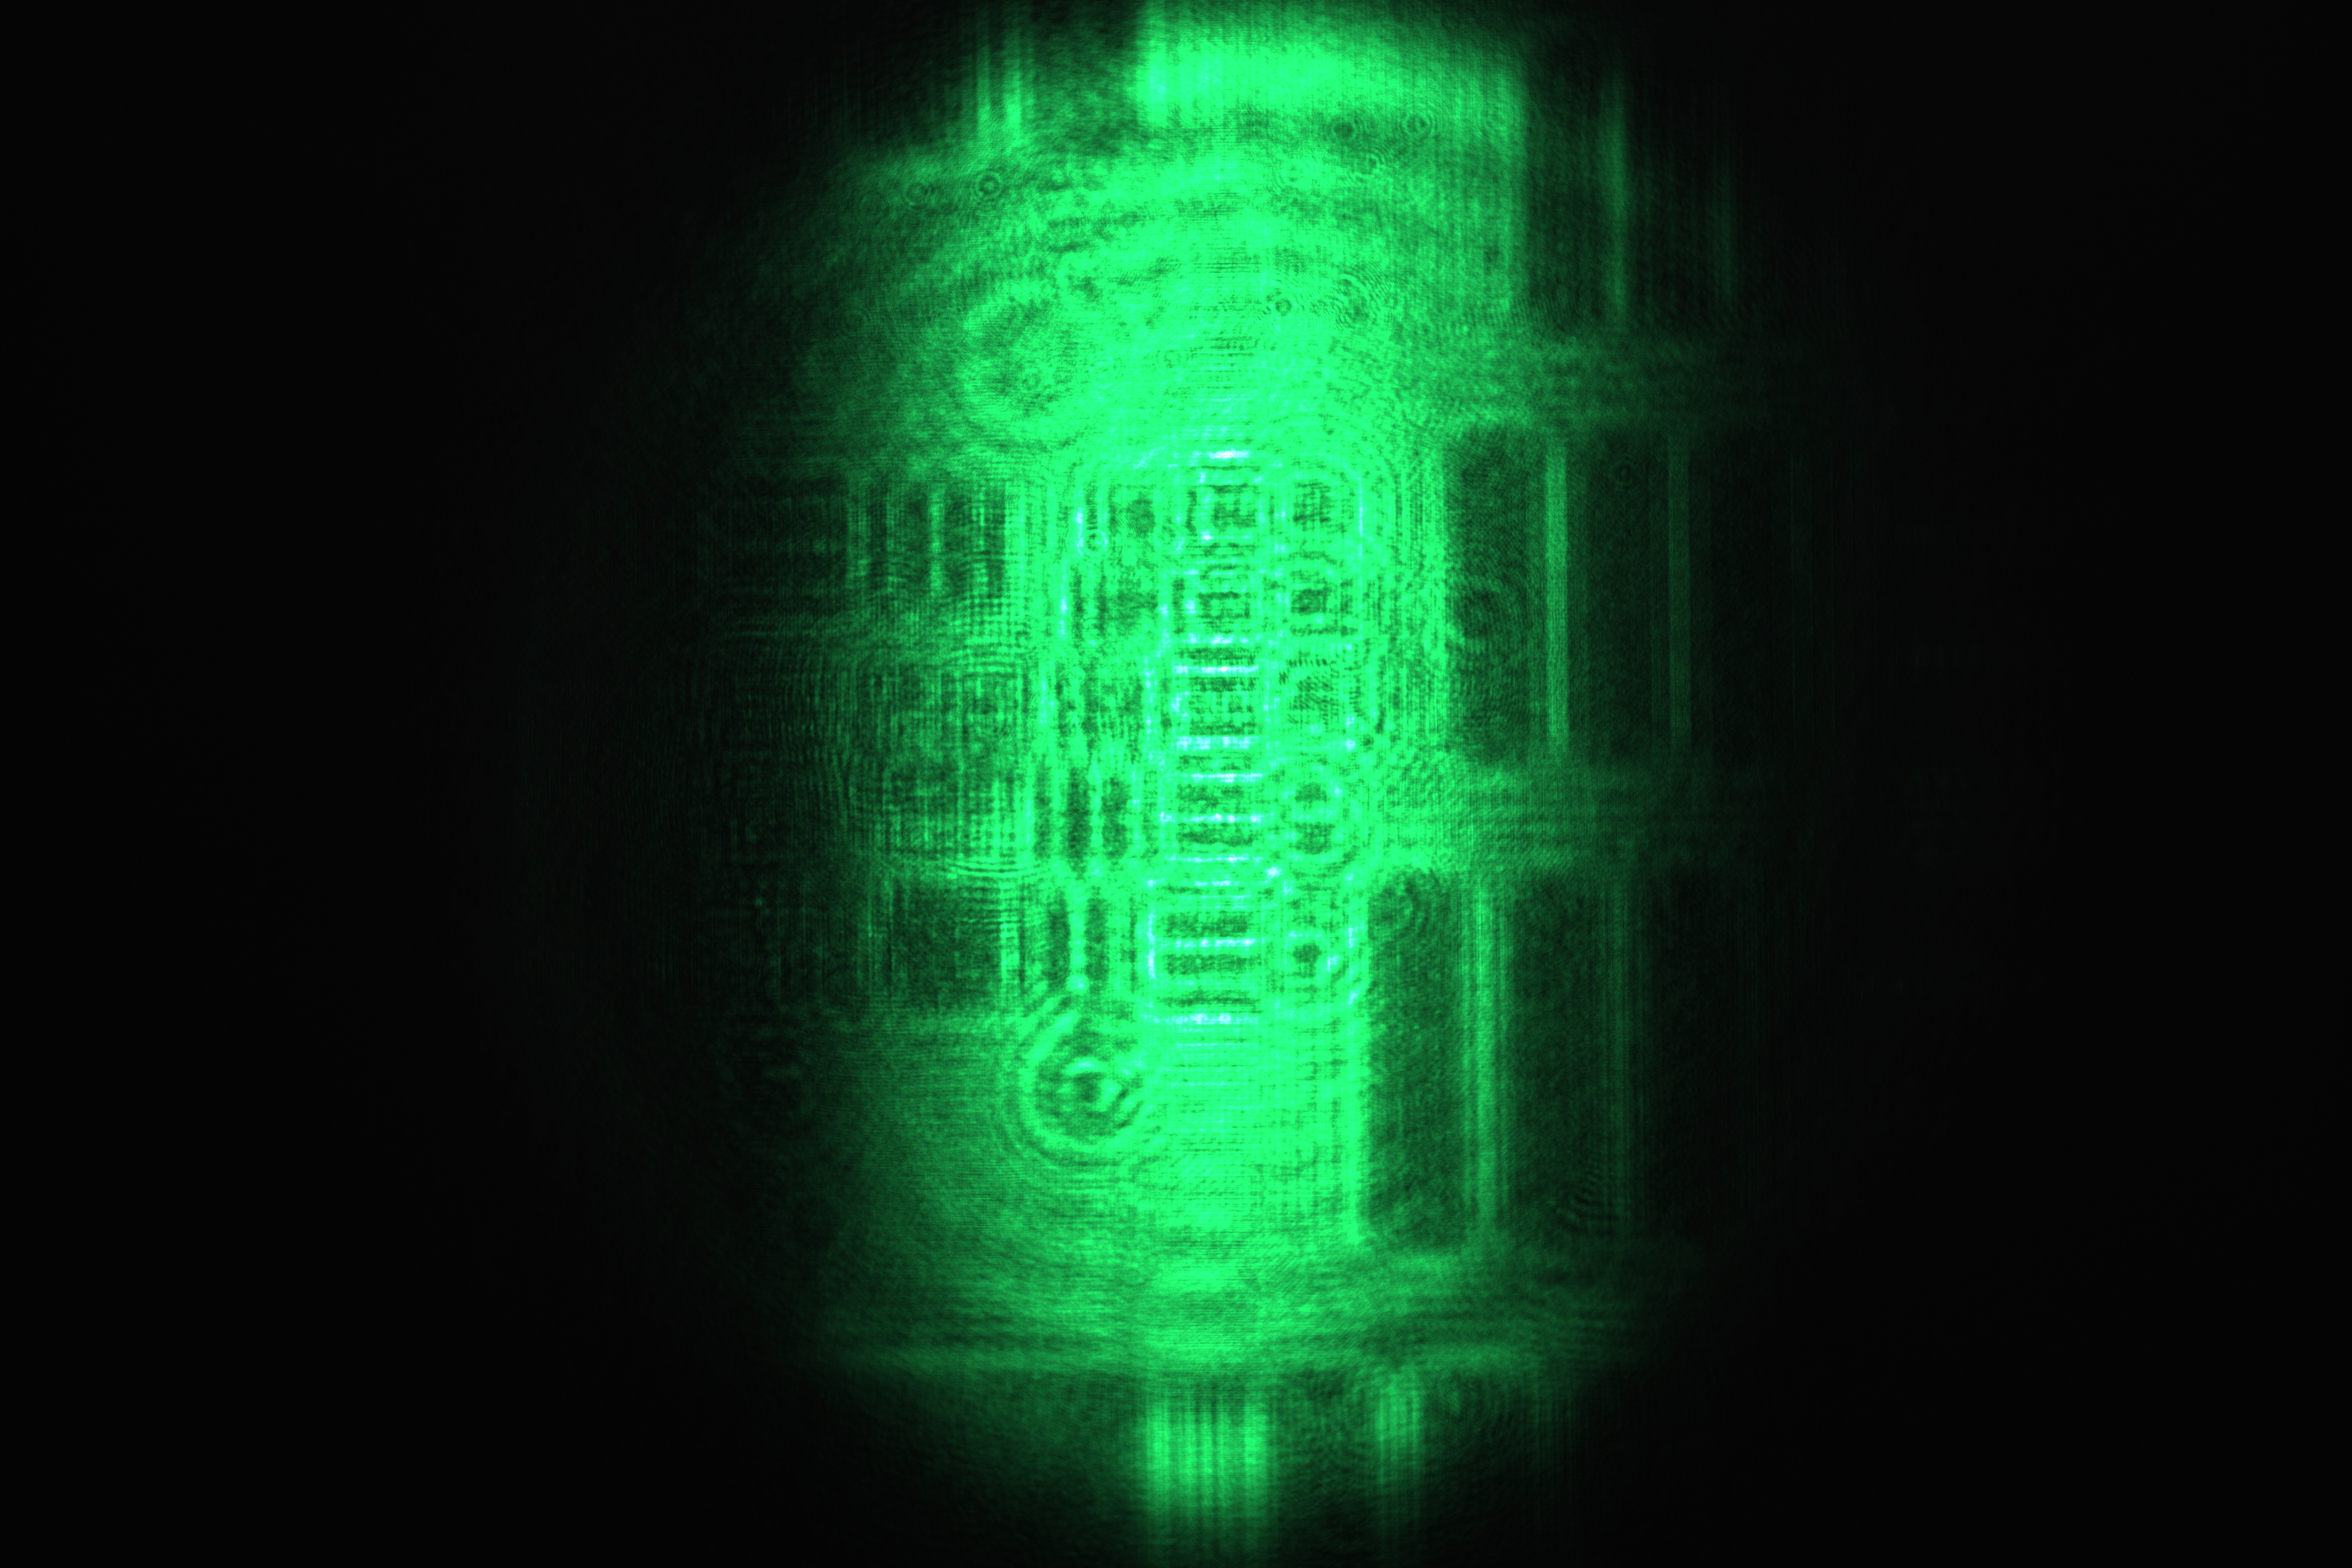
\includegraphics[width=\linewidth]{lizhou2}
    \caption{全息2}
    \label{Fig.sub.2}
\end{subfigure}
\hfill
\begin{subfigure}{0.3\textwidth}
    \centering
    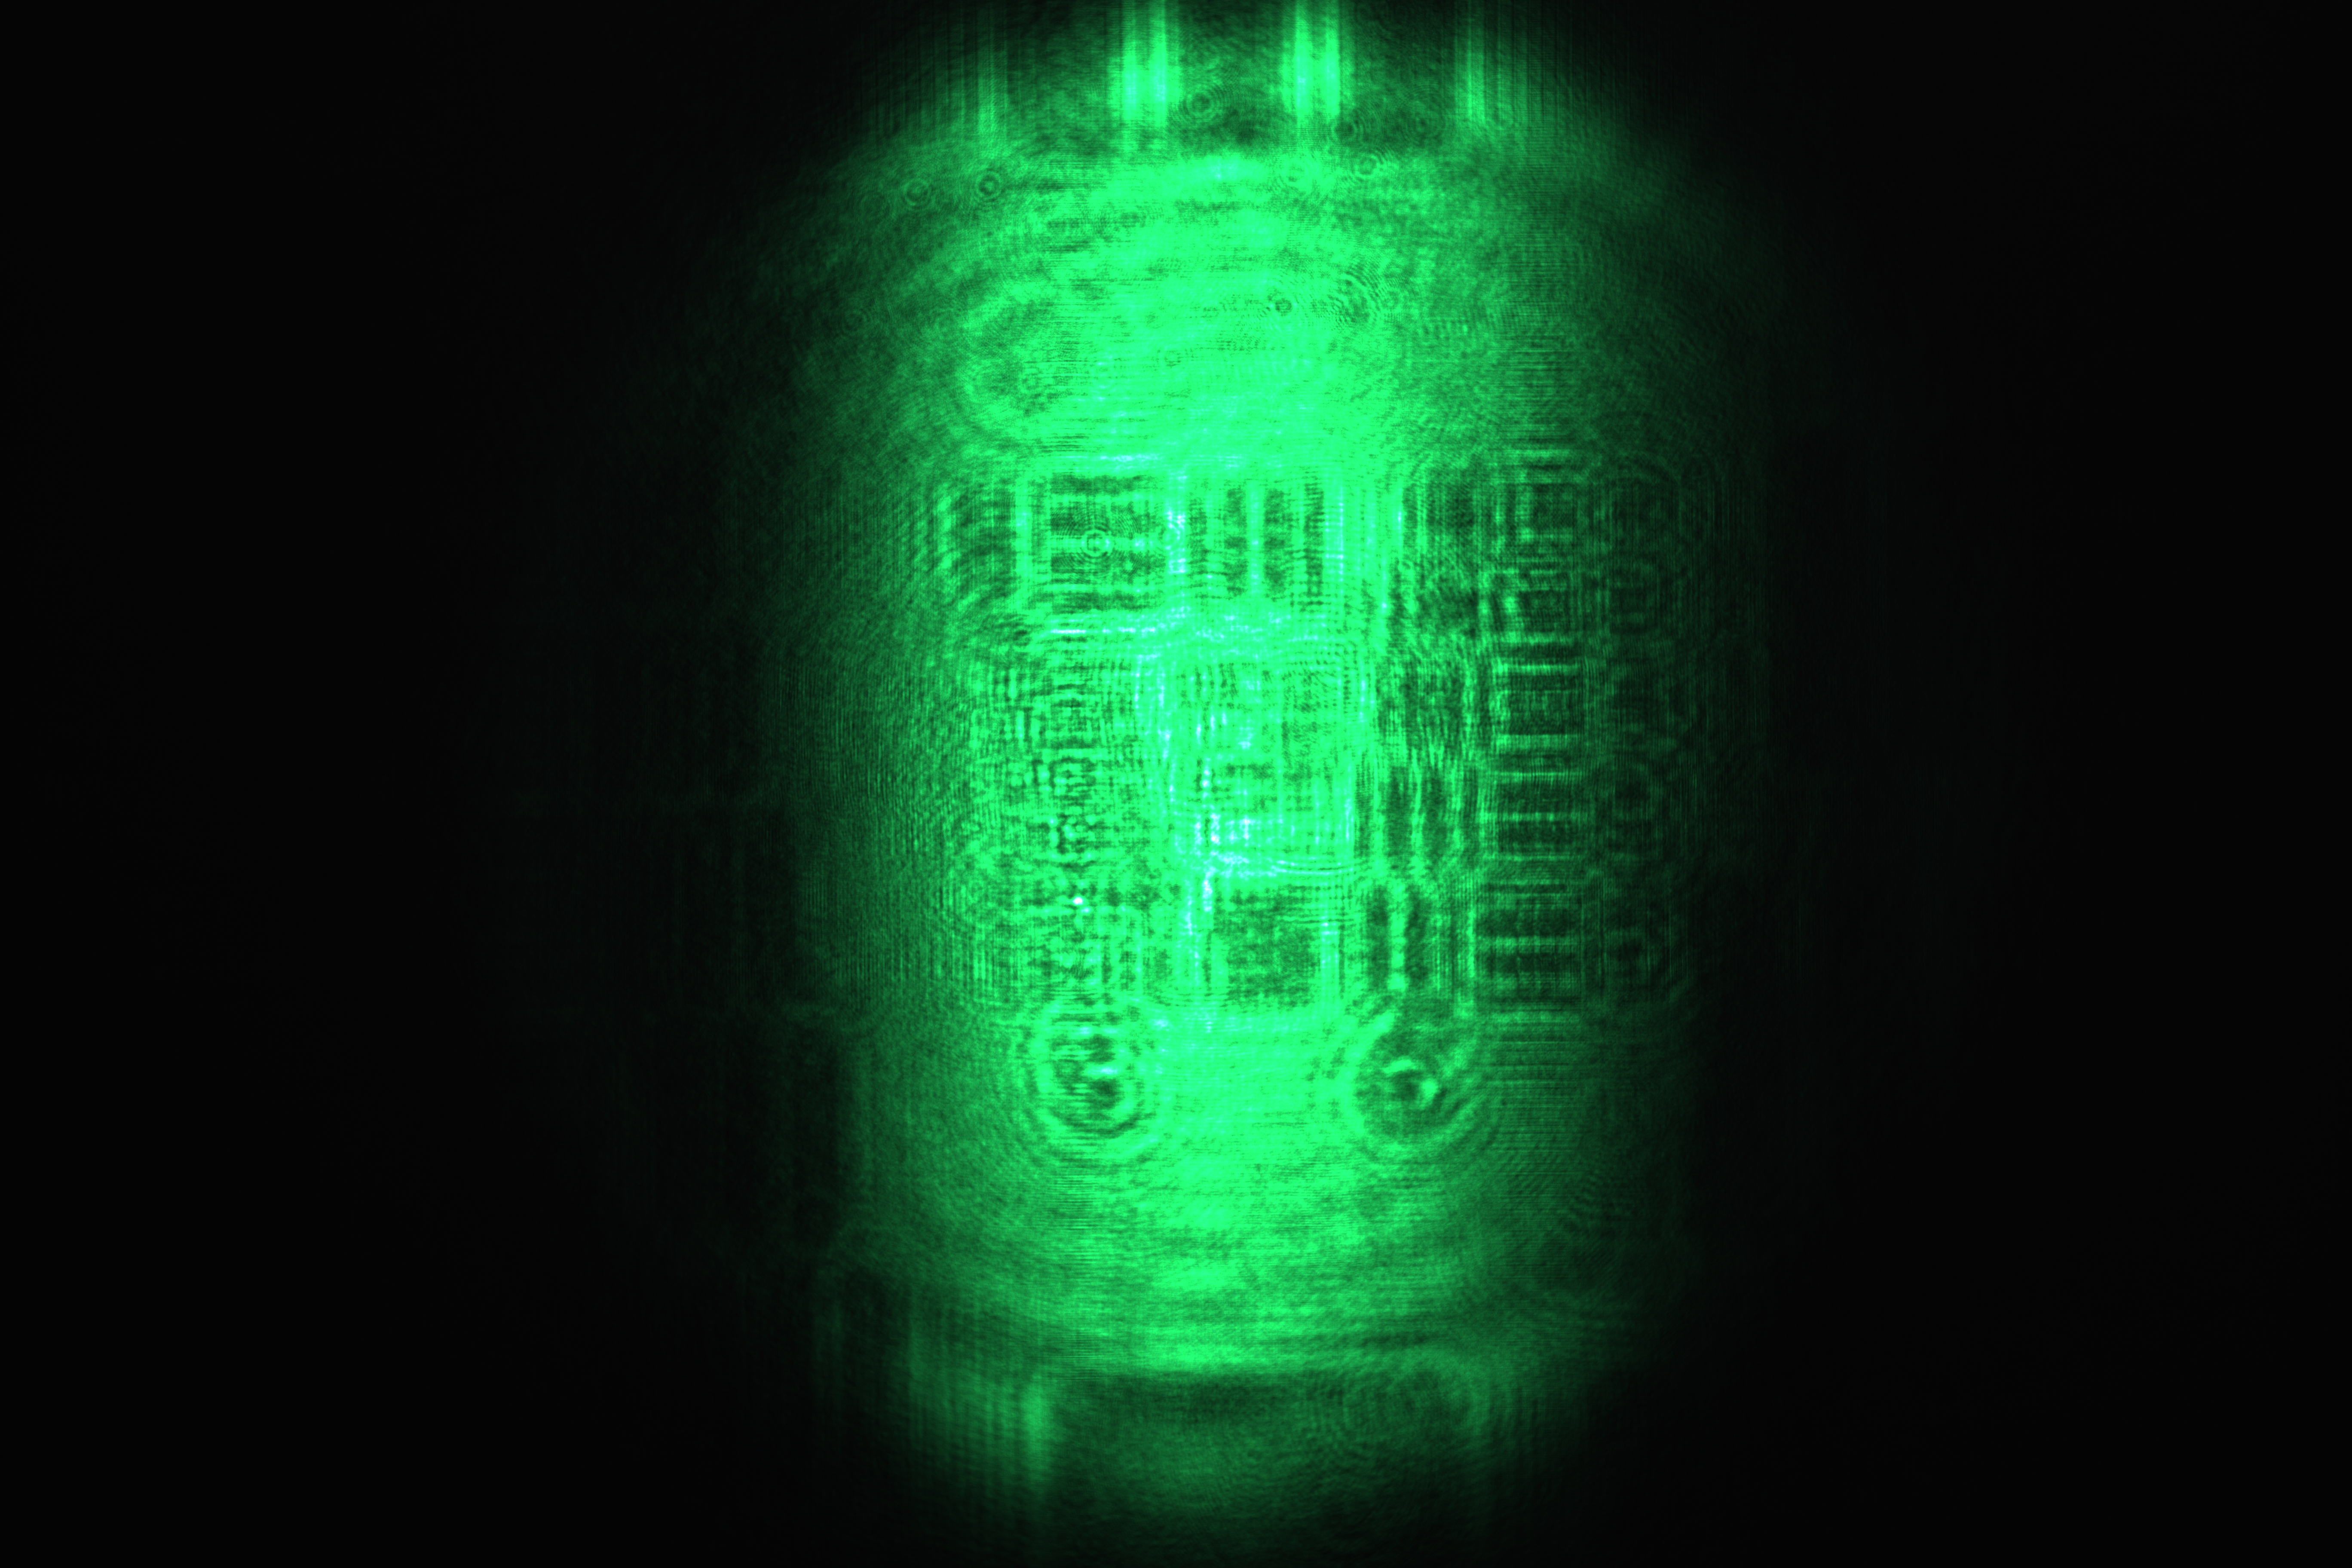
\includegraphics[width=\linewidth]{lizhou3}
    \caption{全息3}
    \label{Fig.sub.3}    
\end{subfigure}

\caption{对分辨率板的不同位置重建并确认距离}
\label{Fig.main1}
\end{figure}
\subsection{重建全息图}
将拍摄的全息图导入计算机,使用Python进行处理。处理过程如下\\
\begin{itemize}
    \item 首先对全息图进行二维傅里叶变换,得到频域图像。
    \item 接着在频域图像中选择合适的带通滤波器,滤除零级像和共轭像的干扰。
    \item 然后对滤波后的频域图像进行逆傅里叶变换,得到物光的复振幅分布。
    \item 使用菲涅尔衍射积分方法,将物光复振幅传播到不同距离,重建出物体在不同位置的图像。
    使用算法评估图像的聚焦程度,在搜索范围内检索每一个z得到一个评价值函数。
    \item 由评价函数最大值对应的z值,作为物体的实际位置的z
\end{itemize}
我们将上述过程集成于一个python程序,只需要将对应图片放入指定文件夹,运行程序即可完成重建。\\
下面是我们使用\ref{Fig.main1}拍摄的全息图进行重建的结果展示,结果中展示了原全息图、确定距离z的过程图
、在最佳距离z重建的重建图和重建图对应的相位分布:
\begin{figure}[H]
\centering
\begin{subfigure}{0.9\textwidth}
    \centering
    \includegraphics[width=\linewidth]{lizhou1分辨率板}
    \caption{离轴1}
    \label{Fig.sub.4}
\end{subfigure}

\begin{subfigure}{0.9\textwidth}
    \centering
    \includegraphics[width=\linewidth]{lizhou2分辨率板}
    \caption{离轴2}
    \label{Fig.sub.5}
\end{subfigure}

\begin{subfigure}{0.9\textwidth}
    \centering
    \includegraphics[width=\linewidth]{lizhou3分辨率板}
    \caption{离轴3}
    \label{Fig.sub.6}    
\end{subfigure}

\caption{对分辨率板的不同位置重建并确认距离}
\label{Fig.main2}
\end{figure}


\chapter{误差分析}

\chapter{结论与展望}

\chapter{参考文献}

\chapter{附录}
\section{人员分工}
\renewcommand{\arraystretch}{1.3} % 表格行距调整
\begin{tabularx}{\textwidth}{>{\bfseries}l X}
\toprule
队员 & 分工 \\
\midrule
队员一 & 负责搭建光路,全息重建的代码,实验报告的撰写。 \\
队员二 & 负责热学相关部分原理的推导和微球布朗运动的模拟。 \\
队员三 & 负责制作ppt和辅助光路搭建。 \\
队员四 & 负责后期数据处理。 \\
\bottomrule
\end{tabularx}

\section{部分代码展示}

\subsection{重建离轴全息}
\begin{lstlisting}[language=Python, caption=离轴全息重建, label=code:generator]
# 这里是代码示例
\end{lstlisting}

\section{部分全息图与拍摄图展示}

\end{document}
